\section{}
\begin{enumerate}

% 2.1 --------------
\item Протон с длиной волны \( \lambda = 1,\!7 \)~пм упруго рассеялся под
углом \( 90^\circ \) на первоначально покоившейся частице, масса которой в
\( n = 4,0 \) раза больше массы протона. Определить длину волы рассеянного
протона.

\emph{Решение:}
    Закон сохранения энергии: 
    \[
        \frac{mv^2}{2} = \frac{mv'^2}{2} + \frac{m_2u^2}{2}.
    \]
    Т.к. \( m_2 = nm \), то \( v^2 = v'^2 + nu^2 \).
    
    По теореме Пифагора: \( (mv)^2 + (mv')^2 = (m_2u)^2 \),
    откуда \( v^2 + v'^2 = (nu)^2 \).
    \[
        \left\{\begin{array}{l}
            v^2 + v'^2 = (nu)^2; \\
            v^2 = v'^2 + (nu)^2.
        \end{array}\right.
    \]
    Решая систему уравнений получаем:
    \[
        v' = v\sqrt\frac{n-1}{n+1}.
    \]
    С учётом соотношения
    \[
        p = \hbar k = \hbar\frac{2\pi}{\lambda} = mv
    \]
    получим
    \[
        \lambda' = \lambda\sqrt\frac{n+1}{n-1}.
    \]

\newpage

% 2.2 --------------
\item Нейтрон с кинетической энергией \( T = 0,\!25 \)~эВ испытал упругое
соударение с первоначально покоившимся ядром атома \( ^4\mathrm{He} \). Найти
длину волн обеих частиц в их Ц-системе до и после соударения.

\emph{Решение:}

\newpage

% 2.3 --------------
\item Два атома, \( ^1\mathrm{H} \) и \( ^4\mathrm{He} \), движутся в одном
направлении, причём дебройлевская длина волны каждого атома
\( \lambda = 60 \)~пм. Найти длины волн обоих атомов в их Ц-системе.

\emph{Решение:}

\newpage

% 2.4 --------------
\item Найти кинетическую энергию электронов, падающих нормально на диафрагму с
двумя узкими щелями, если на экране, отстоящем от диафрагмы на \( l = 75 \)~см,
расстояние между соседними максимумами \( \Delta x = 7,\!5 \). Расстояние между
щелями \( d = 25 \)~мкм.

\emph{Решение:}

\newpage

% 2.5 --------------
\item Узкий пучок моноэнергетических электронов падает под углом скольжения
\( \theta = 30^\circ \) на грань монокристалла алюминия. Расстояние между
соседними кристаллическими плоскостями, параллельными этой грани монокристалла,
\( d = 0,\!20 \)~нм. При ускоряющем напряжении \( U_0 \) наблюдали максимум
зеркального отражения. Найти \( U_0 \), если следующий максимум зеркально
отражения возникал при увеличении ускоряющего напряжения в
\( \eta = 2,\!25 \)~раза.

\emph{Решение:}

\newpage

% 2.6 --------------
\item Узкий пучок электронов с кинетической энергией \( K = 10 \)~кэВ проходит
через поликристаллическую алюминиевую фольгу, образуя на экране систему
дифракционных колец. Вычислить межплоскостное расстояние, соответствующее
отражению третьего порядка от некоторой системы кристаллических плоскостей, если
ему отвечает дифракционное кольцо диаметра \( D = 3,\!20 \)~см. Расстояние между
экраном и фольгой \( l = 10,\!0 \)~см.

\emph{Решение:}
    \begin{align*}
        &\ \Delta = d\sin\varphi; \\
        \Delta =\ &n\lambda = \frac{2n\pi\hbar}{p} = \frac{2n\pi\hbar}{\sqrt{2mT}}; \\
        & d\sin\varphi = \frac{2n\pi\hbar}{\sqrt{2mT}}; \\
        & d = \frac{2n\pi\hbar}{\sqrt{2mT}\sin\varphi}.
    \end{align*}

\newpage

% 2.7 --------------
\item Интерпретировать квантовые условия Бора на основе волновых представлений:
показать, что электрон в атоме водорода может двигаться только по тем круговым
орбитам, на которых укладывается целое число дебройлевских волн.

\emph{Решение:}
    \begin{align*}
        \lambda = \frac{h}{p}; \quad p = &\ mv = \frac{h}{p\lambda}. \\
        % импульс = h/(lambda*импульс)? WAT
        mv(2\pi R) = &\ \frac{h}{p\lambda}(2\pi R); \\
        mv(2\pi R) & = hn.
    \end{align*}
    Условие квантования: \( pRmv = nh/(2\pi) \)
    \[
        \frac{h}{p\lambda}(2\pi R) = nh;\quad
        2\pi R = n\lambda;\quad
        R = \frac{n\lambda}{2\pi}
    \]

\newpage

% 2.8 --------------
\item Убедиться, что измерения координаты частицы с помощью микроскопа вносит
неопределенность в её импульс \( \Delta p_x \), такую, что
\( \Delta x\cdot\Delta p_x \ge h \). Иметь в виду, что разрешение микроскопа
\( d = \lambda/\sin\theta \), где \( \lambda \) -- длина волны используемого
света.

\emph{Решение:}
    \begin{table}[h!]
    \begin{tabular}{m{.55\textwidth}C{.4}}
    У фотона, рассеянного на микрочастице и прошедшего через объектив O,
    проекция импульса \( p_x \) не превышает, как видно из рисунка \smiley,
    значение \( p\sin\theta = \hbar k\sin\theta \), где \( k = 2\pi/\lambda \).
    Эта величина характеризует и неопределенность \( \Delta p_x \) фотона. Но
    при рассеянии фотона на микрочастице последняя испытывает отдачу, в
    результате чего её импульс получит такую же неопределенность \( \Delta p_x\),
    как и фотон: \( \Delta p_x \approx \hbar k\sin\theta \).
    
    Имея, кроме того, в виду, что неопределенность координаты \( x \)
    микрочастицы \( \Delta x \approx d = \lambda/\sin\theta \),
    & 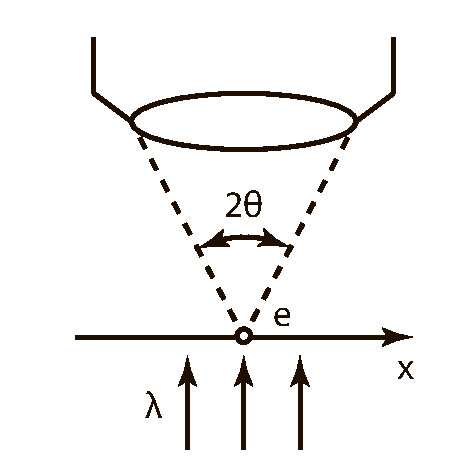
\includegraphics[height=15em]{2_08}
    \end{tabular}
    \end{table}
    
    получим в результате:
    \[ 
        \Delta x\cdot\Delta p_x \approx \frac{\lambda}{\sin\theta}
        \frac{2\pi\hbar}{\lambda}\sin\theta = 2\pi\hbar
    \]
    в чём и следовало убедиться.

\newpage

% 2.9 --------------
\item Плоский поток частиц падает нормально на диафрагму с двумя узкими щелями,
образуя на экране дифракционную картину. Показать, что попытка определить, через
какую щель прошла та или иная частица (например, с помощью введения индикатора
И), приводит к разрушению дифракционной картины. Для простоты считать углы
дифракции малыми.

\emph{Решение:}
    \begin{table}[h!]
    \begin{tabular}{m{.5\textwidth}C{.45}}
    & 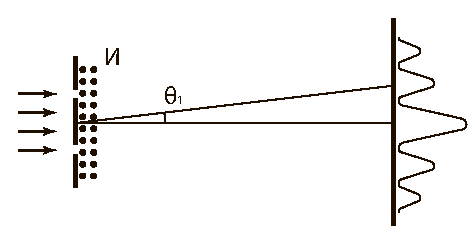
\includegraphics{2_09}
    \end{tabular}
    \end{table}

\newpage

% 2.10 -------------
\item Оценить минимально возможную энергию электронов в атоме Не и
соответствующее расстояние электронов от ядра.

\emph{Решение:}

\newpage

% 2.11 -------------
\item Оценить с помощью соотношения неопределенностей неопределенность скорости
электрона в атоме водорода, полагая размер атома \( l = 0,\!10 \)~нм. Сравнить
полученную величину со скоростью электрона на первой боровской орбите данного
атома.

\emph{Решение:}

\newpage

% 2.12 -------------
\item Оценить с помощью соотношения неопределенностей минимальную кинетическую
энергию электрона, локализованного в области размером \( l = 0,\!20 \)~нм.

\emph{Решение:}

\newpage

% 2.13 -------------
\item Электрон с кинетической энергией \( T \approx 4 \)~эВ локализован в
области размером \( l \approx 1 \)~мкм. Оценить с помощью соотношения
неопределенностей относительную неопределенность его скорости.

\emph{Решение:}

\newpage

% 2.14 -------------
\item Электрон находится в одномерной прямоугольной потенциальной яме с
бесконечно высокими стенками. Ширина ямы \( l \). Оценить с помощью соотношения
неопределенностей силу давления электрона на стенки этой ямы при минимально
возможной его энергии.

\emph{Решение:}

\newpage

% 2.15 -------------
\item След пучка электронов на экране электронно-лучевой трубки имеет диаметр
\( d \approx 0,\!5 \)~мм. Расстояние от электронной пушки до экрана
\( l \approx 20 \)~см, ускоряющее напряжение \( U = 10 \)~кВ. Оценить с помощью
соотношения неопределенность координаты электрона на экране.

\emph{Решение:}

\newpage

% 2.16 -------------
\item Частица массы \( m \) движется в одномерном потенциальном поле
\( U = \cfrac{\chi x^2}{2} \) (гармонический осциллятор). Оценить с помощью
соотношения неопределенностей минимально возможную энергию частицы в таком поле.

\emph{Решение:}

\newpage

% 2.17 -------------
\item Параллельный пучок атомов водорода со скоростью \( \nu = 600 \)~м/с падает
нормально на узкую щель, за которой 	на расстоянии \( l = 1,\!0 \)~м расположен
экран. Оценить с помощью соотношения неопределенностей ширину \( b \) щели, при
которой ширина изображения её на экране будет минимальной.

\emph{Решение:}

\end{enumerate}
